\documentclass{article}

\usepackage[utf8]{inputenc}

\usepackage{graphicx}
\graphicspath{{images/}}

\renewcommand{\familydefault}{\sfdefault}
\usepackage[a4paper]{geometry}

\usepackage{listings}
\lstset{language=SQL}

\usepackage{tcolorbox}
\newtcolorbox{keypointbox}
{
    arc=0mm,
    colback=red!20,
    colframe=red!80,
    leftrule=5pt,
    toprule=0pt,
    rightrule=0pt,
    bottomrule=0pt
}

\setcounter{secnumdepth}{2}

\usepackage{hyperref}
\usepackage{cleveref}

\title{Data Warehouse Systems}
\author{Alexander Schlögl}

\begin{document}
\maketitle

\tableofcontents

This is \textbf{my interpretation} of the lecture slides.
I tried to be very verbose and explain everything, all while removing irrelevant parts from the lecture.
Using this you should be able to pass the lecture easily.
\large{\textbf{However, I do not take responsibility for any bad results and will not be blamed from anyone.
This was a lot of work and I did it to save others (especially students of following semesters) from having to do this themselves.
Use this summary at your own responsibility.}}
If you have any feedback, feel free to create an issue on the \href{https://github.com/alxshine/lecture-notes}{git}.
I don't promise I will fix anything, but I will try.
\newpage

\section{Definition}
\textbf{GI-Group Definition:}
“A Data Warehouse is a database which (from a technical point of view) integrates data from different (heterogeneous) data sources and (from an economic point of view) provides the user with this data for business analysis purposes. Frequently, but not necessarily, a historization of data takes place.”
\\
\textbf{Inman's Definition:}
“A data warehouse is a subject-oriented, integrated, time-variant and non-volatile collection of data in support of management's decision making process.”
\textbf{Integrated} means the data is collected from multiple (separate) sources, and compiled into a single source of truth.
\textbf{Time-variant} means that the data is accurate at the time it was compiled (ie. the transactions took place).
This is very useful for observing changing trends.
\textbf{Non-volatile} means the compiled data in the DWS is not changed (often), but only queried.
\begin{keypointbox}
    A DWS is a static copy of accumulated transaction data used for analysis.
\end{keypointbox}

Data Warehouses are not single products, but a system comprised of multiple interacting components, most of which are usually bought from third-parties.

\subsection{Operational Data Stores vs. Data Warehouses}
Operational Data Stores (ODSs) are used in the day to day transactions of a business.
They are very fast, use a single data source, are used by multiple users concurrently and mostly perform small transactions (e.g. sales).
Think of the database interacting with Point of Sale terminals in a supermarket.

Data Warehouse (DWs) are very large databases used to store accumulated data.
They are usually only accessed by single users and even then mostly only for reads.
Data is fed into DWs periodically (e.g. daily or weekly), and then usually not changed afterwards.
This means that locks can be optimized differently for DWs than for ODSs.
The access patterns are also very different from ODSs, with range queries being the norm.

A full comparison is given in \Cref{tbl:odsDwComp}.

\begin{table}[ht]
    \center
    \begin{tabular}{| l | l | l |}
        \hline
        & ODS & DW\\
        \hline
        Data Sources & mostly only one & many\\
        Data Volume & MB-GB & GB-TB-PB\\
        Access & Single Tuple accesses & Range queries\\
        Up-to-dateness & Up to date & (Possibly) outdated\\
        Use & Input output by employees & Evaluation by analysts/managers\\
        Number of users & Many & few\\
        Response time & ms-s & s-min-h\\
        \hline
    \end{tabular}
    \caption{Comparison between ODSs and DWs}
    \label{tbl:odsDwComp}
\end{table}

\begin{keypointbox}
    ODSs are regular databases.
    DWs are larger, and optimized for range-queries and rare modifications.
\end{keypointbox}

\begin{keypointbox}
    ODSs are used for Online Transaction Processing (OLTP), and DWs for Online Analytics Processing (OLAP).
\end{keypointbox}

\section{Reference Architecture}
\label{architecture}
The goal of a reference architecture is to provide a fundamental, abstract, implementation independent visualization of the DW.
It is useful for comparing DW models, systems and components and can be used for planning specifications and implementations of a DW system.
A reference architecture should provide an overview of the operators (functions) and operands (databases, data), as well as the \textbf{data-flow} required for the functions and the \textbf{control-flow} required for the underlying processes.

\begin{keypointbox}
    A reference architecture is a model of a DW system.
\end{keypointbox}

\subsection{Requirements of a DW architecture:}
\begin{itemize}
    \item \textbf{Isolation:} the DW should be independent of its data sources after the data has been imported.
    \item \textbf{Persistency:} after importing the data the DW should suffice as a permanent storage
    \item \textbf{Flexibility of use:} arbitrary evaluations should be possible
    \item \textbf{Scalability:} it should be easy to integrate new data sources over time
    \item \textbf{Efficiency:} repeating tasks should be easy to automate
    \item \textbf{Uniqueness} of data structures, access rights and processes
    \item \textbf{Orientation} of the system towards the analysis of data (ie. optimizations for range queries)
\end{itemize}

\subsection{Static View of a DW Architecture}
This is a view of the static components themselves, ie. the databases or the component extracting data from data sources.
The system components include:
\begin{itemize}
    \item \textbf{Interface components:} DW manager, Metadata manager
    \item \textbf{Databases:} DW, Base DB, Metadata DB
    \item \textbf{Functional components:} Monitor, Extraction, Transformation, Loading and Analysis components
\end{itemize}

The static view is (somewhat) equivalent to the white blobs in \Cref{fig:flow}.

\subsection{Dynamic View of a DW Architecture}
The dynamic view contains the data flow (comprised of main- and metadata flow) as well as the control flow.
It is depicted by the arrows in \Cref{fig:flow}, with the solid arrows being data-flow and the dashed arrows being control-flow.

\begin{figure}
    \center
    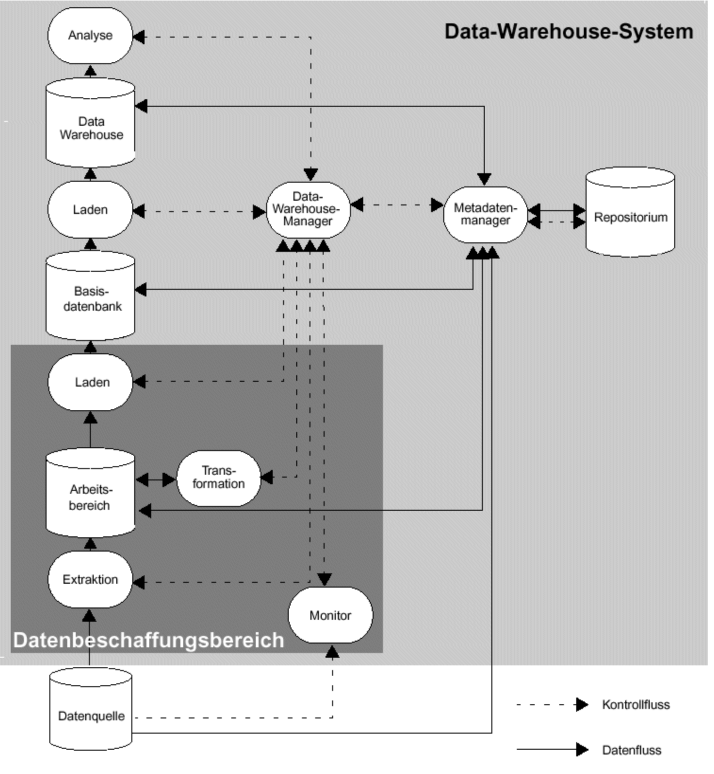
\includegraphics[width=0.8\textwidth]{control_flow.png}
    \caption{The data and control flow from a data source to the DW}
    \label{fig:flow}
\end{figure}

\subsection{Components of a DW System}
\begin{keypointbox}
    All the DW components do exactly what their name suggests.
    \Cref{fig:flow} is in principle enough to fully understand \Cref{architecture}.
\end{keypointbox}

The \textbf{monitor} handles the extraction from the data source(s), sometimes filtering out irrelevant data.
Relevant data is extracted into the (temporary) \textbf{working area}, where it is \textit{transformed} (cleaned, integrated, etc.).
To reduce potential consistency issues caused by changing dimension data (e.g. product names changing), the data can then be loaded into a \textbf{base database}.
This database contains the raw transformed data, which needs to be combined with metadata to be meaningful.
The base database is application independent and modelled based on the relations in the data.
Finally, the data can be combined with metadata and loaded into the \textbf{data warehouse} which is modelled specifically for the application (analysis).
The metadata is kept in a separate metadata \textbf{repository}.

\subsection{Data Sources}
The selection of data sources for the data warehouse is a defining factor for the quality of the finished data warehouse.
Sources must be selected based on their \textbf{relevance} and the \textbf{quality of their data}.
Factors for relevance are:
\begin{itemize}
    \item Purpose of the data warehouse
    \item Availability of the source data (technical, organisational, legal)
    \item Cost of acquisition
\end{itemize}
Factors for quality are:
\begin{itemize}
    \item Correctness
    \item Consistency
    \item Completeness
    \item Comprehensability (Metadata, documentation)
\end{itemize}

Data sources can also be classified based on a number of characteristics; examples include origin, time, usage (metadata, base-data), ...

\subsection{Control Components}
Important control components are:

The \textbf{data warehouse manager} handles initialization, control and management of all functions and other components.
It is the main control component and manages the entire work- and data-flow.

The \textbf{metadata manager} does exactly what the name says.
It manages metadata, including start and end dates of validity (important for renames and the like) and links between the data warehouse manager and the metadata repository.

\textbf{Monitors} are used (one per data source) to monitor for updates and extract new data.
They can either directly feed relevant data to the work area, or simply notify the manager of updates and wait for scheduled extraction.
Techniques for extracting are \textit{trigger-based} (periodically, ...), \textit{replication-based} (store changed tuples in special relation), \textit{timestamp-based}, \textit{log-based}, \textit{snapshot-based} (operate on deltas, high implementation effort but sometimes only possibility for legacy systems).

\subsection{Work Area}
It is a temporary storage area required for the process of data transformation, and the central storage for \textbf{ETL-components}.

\subsection{ETL-Components}
ETL stands for extraction, transformation and loading, and describes the components needed in order to fill the data warehouse with data originally from the data sources.
As the data sources are heterogeneous (e.g. different currencies, incosistent schemas, ...) the data needs to be cleaned and annotated with metadata in order to be useful.
This cleanup is done in the ETL process.

\subsubsection{Extraction Component}
Controls the periodical transmission of source data to the working area.
The extraction time determines the analysis accuracy and depends on the analysis goals.
Examples for times the extraction can take place are:
\begin{itemize}
    \item periodical
    \item on demand
    \item event-driven
    \item immediately on updates
\end{itemize}
The extraction strategy dictates the extraction techniques.

\subsubsection{Transformation Component}
Transformation is the process of reshaping the schema (column names, ...) as well as cleaning the data and unifying data types, currencies, unit formats (times, ...) etc.

During this process the data is also checked for integrity violation, illegal values (consistency and plausibility checks), redundancy, incomprehensible and inconsistent values, as well as missing and NULL values.
All these checks are part of the code cleanup.

The schema transformation that is done by this component is necessary due to a heterogenity of the data sources.
Because different data sources have different views, legal requirements or simply different models their schemas can vary wildly.
Schema transformation requires expert knowledge and is hard to automate, as a transformation script has to be created for every single data source.
It also requires the setup of the metadata database.

\Cref{fig:transformation} shows the individual steps of the transformation process.

\begin{figure}[hp]
    \centering
    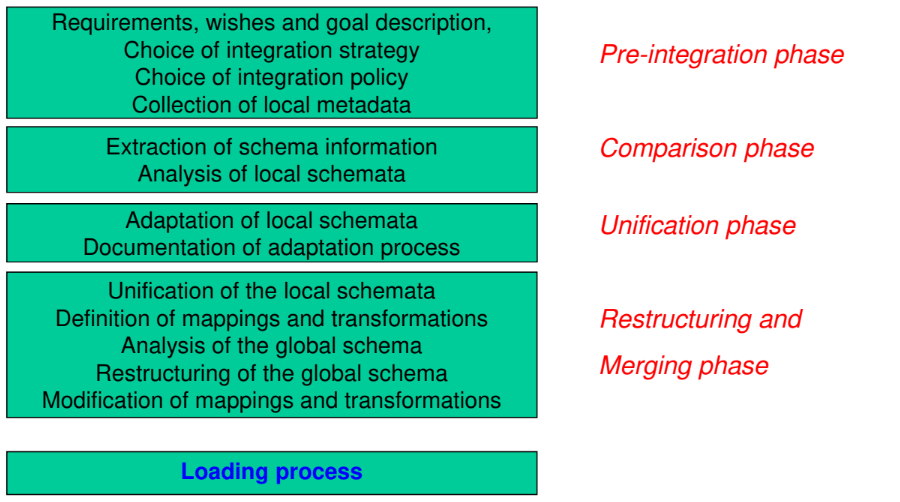
\includegraphics[width=0.8\textwidth]{transformation.png}
    \caption{The steps of the transformation process}
    \label{fig:transformation}
\end{figure}

\subsubsection{Loading Component}
This component takes care of loading the transformed data into the database(s).
If there is no base database the analytics specific data is transmitted to the data warehouse from the working area.
If such a database does exist, the cleaned data is loaded into it, and a version of the data made specifically for analysis is sent to the data warehouse.
The anlysis version might include pre-aggregated results.

\subsection{Base Database}
The base database acts as a \textbf{central data storage}.
It stores the cleaned data at the highest resolution (lowest granularity) while staying completely application netral.
It functions as a buffer between the data sources and data warehouses.

In a situation where there are multiple DWs the base database functions as the \textbf{single source of truth}, thus saving the DWs from gathering their data from each data source themselves.
This reduces complexity from $\mathcal O (m \cdot n)$ to $\mathcal O (m + n)$.

The documentation of the base database must ensure traceability for the entire data flow from the sources to the base database.
This includes the ETL process and points of possible human intervention in case the automated system fails.
The documentation of the ETL processes must be \textbf{exact} so they can be reproduced in the next iteration.

The metadata repository as well as the base database must be \textbf{available} for the DWs to function properly if they are the single source of truth.

\subsection{Data Warehouse}
The DW is specifically organized for analysis.
This includes ordering along multiple dimensions.
In order to speed up this sorting, DWs have moved to multi-dimensional representations of their data.

Special requirements for a database management system (DBMS) of a DW include:
\begin{itemize}
    \item bulk loading
    \item access interface for analysis tools
    \item Optimization and tuning for frequent queries (indices, materialized views, ...)
\end{itemize}

\subsection{Data Marts}
Data marts provide a partial view of the DW.
They can either access the DW for data (requiring a permanent connection) or save their relevant part themselves.
Both variants come with a tradeoff of availability versus integrity.

Splitting the DW into multiple data marts allows departments to operate independent of each other, as well as distributing the workload and required storage.

Data marts can be categorized by geography, organisation or function.
While they can be kept independent from the main DW by gathering the data directly after the ETL process, this causes a lot of integrity problems and \textbf{should be avoided}.

\subsection{Metadata Repository}
The metadata repository contains a description of the \textbf{entire} DW system.
This includes information about schemata, data-types, formats, but also the setup, maintenance and adminstration of the DWS itself.
It is vital for understanding the data, and without it, the base database is essentially worthless.

The repository is managed by the metadata manager component.

\subsection{Analysis tools}
Analysis tools are also called Business Intelligence (BI) tools, and operate on the DW.
They can be classified by their intended use into reporting tools, OLAP tools (used for interactive data analysis), and data mining tools (used for finding patterns in the data).

\subsubsection{OLAP systems}
These systems are used for online analytics.
Cobb (inventor of database management), defines twelve rules for a good OLAP system, which are extended in the lecture slides to 18:
\begin{enumerate}
    \item Conceptional multi-dimensional view
    \item Transparency for access from multiple data sources (Transparency in this case means that the extra steps taken for the access to a different data source are invisible (transparent) to the user, not that the access is easy to understand)
    \item Flexible access possibilities
    \item Same response time in report creation (in regard to queries on different dimensions)
    \item Client-Server architecture
    \item Equality of dimensions
    \item Adaptive administration of sparse data cubes
    \item Multi-user operation
    \item Unlimited, cross-dimensional operations
    \item Intuitive data handling
    \item Flexible reporting
    \item Unlimited number of dimensions/aggregation levels
    \item Easy data integration
    \item Support of different analysis models
    \item Separation of analysis and operative data
    \item Separation of storage areas
    \item Differentiation between NULL and non-existant values
    \item Handling of missing values
\end{enumerate}

\section{Multi-dimensional Data Modeling}
As we usually want aggregations along multiple dimensions in DWSs, we want our (conceptual) model to represent this.
Therefore we need to adapt existing modeling methods for multiple dimensions.
While our representation of the data is multi-dimensional, internally all data is still stored in relational databases, so our adapted modeling methods are very related to traditional relational modeling methods.
A comparison can be found in \Cref{fig:modeling}.

\begin{figure}[h]
    \centering
    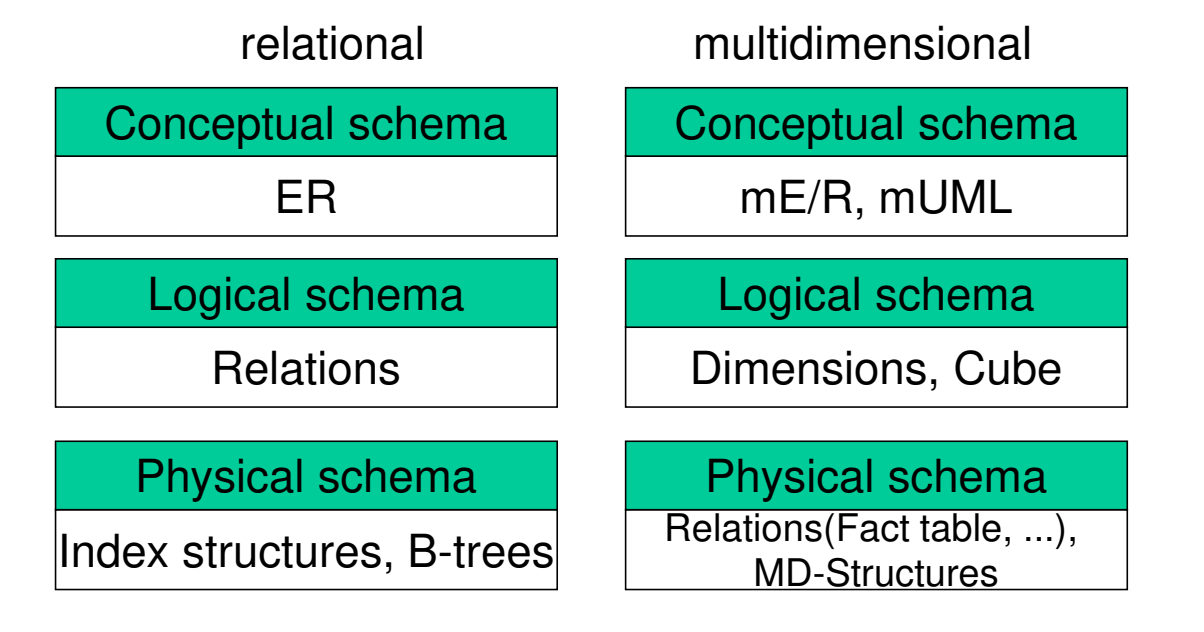
\includegraphics[width=0.6\textwidth]{modeling.png}
    \caption{A comparison of relational and multi-dimensional modeling methods}
    \label{fig:modeling}
\end{figure}

\begin{keypointbox}
    Multi-dimensional modeling works just like regular modeling.
    If you understand ER diagrams, creating mER diagrams is easy, just add multiple hierarchies.
    An example can be found in \Cref{fig:schema}.
\end{keypointbox}

\subsection{Schemas and Instances}
A classification schema (of a dimension) is a set $D$ of classification levels: $(\{D_0, ..., D_{top}\}, \rightarrow)$.
Together with their dependency operator $\rightarrow$ they become a partially ordered set (the partial order allows for multiple parallel hierarchies).
Dimension elements are occurences of the lowest classification level $D_0$ and occurences of higher classification levels are hierarchy nodes.
Three examples for a classification schema can be found in \Cref{fig:schema}.
Every path from $D_0$ to $D_{top}$ defines a classification hierarchy, and a instance of a dimension is the set of all classification hierarchies.

\begin{figure}[h]
    \centering
    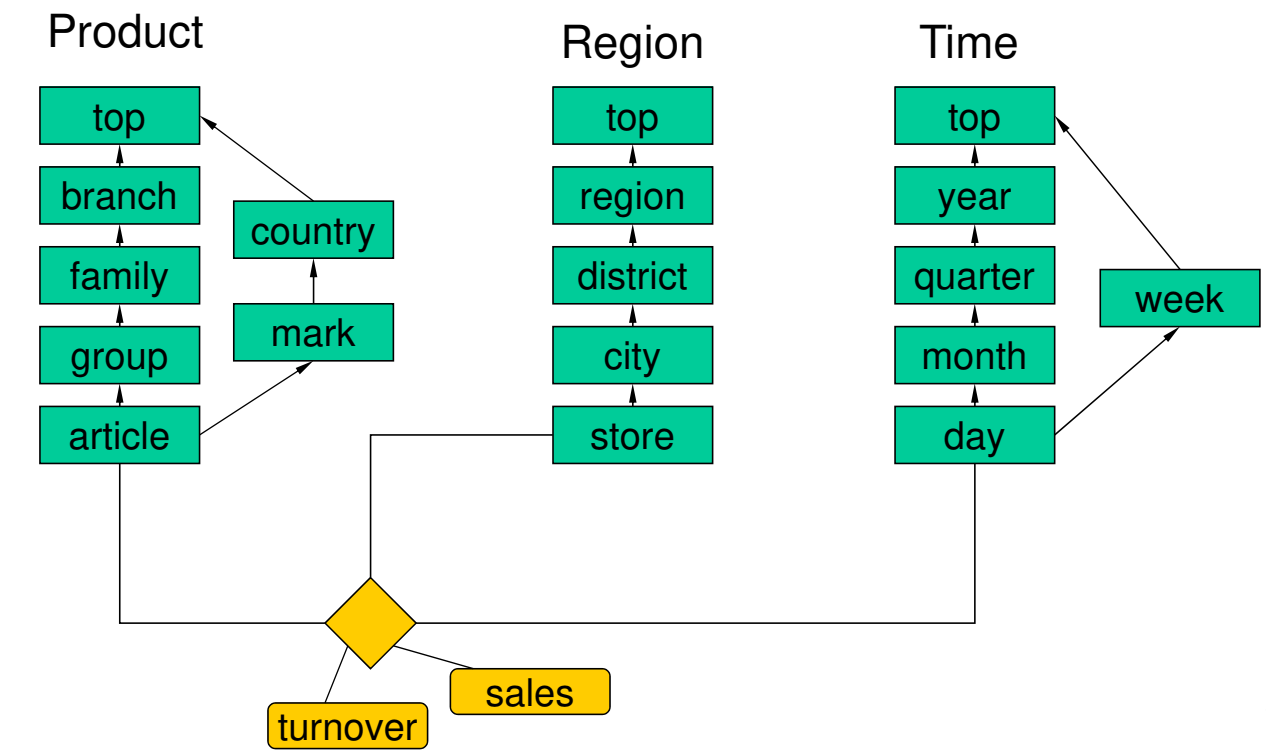
\includegraphics[width=0.8\textwidth]{schema.png}
    \caption{An example for a mER diagram with multiple classification schemes}
    \label{fig:schema}
\end{figure}

\subsection{Data cubes}
As the highest number of dimensions we can easily visualize as a geometrical shape is three, data cubes are a common representation of higher-dimensional data.
The cube consists of data cells which contain $1$ to $n$ measures, and the location in the cube along its three axes represents the values along three dimensions (e.g. geographical, time and product).

\subsubsection{Cube Schemas and Instances}
A cube schema $W\left[G,M\right]$ consists of the granularity $G$ and the set of measures $M$.
For example, if we were to store the sales of an article per store and per day, $G$ would be the set of article, store and day.
Our measures $M$ would be the sales and maybe additionally the turnover.

An instance of a cube $W$ contains all cells from the definition domain of the cube $W = dom(G) \times dom(M)$.
In general, not all cells have a value.
\Cref{fig:cube} shows an instance of a cube including classification hierarchies.

\begin{figure}[h]
    \centering
    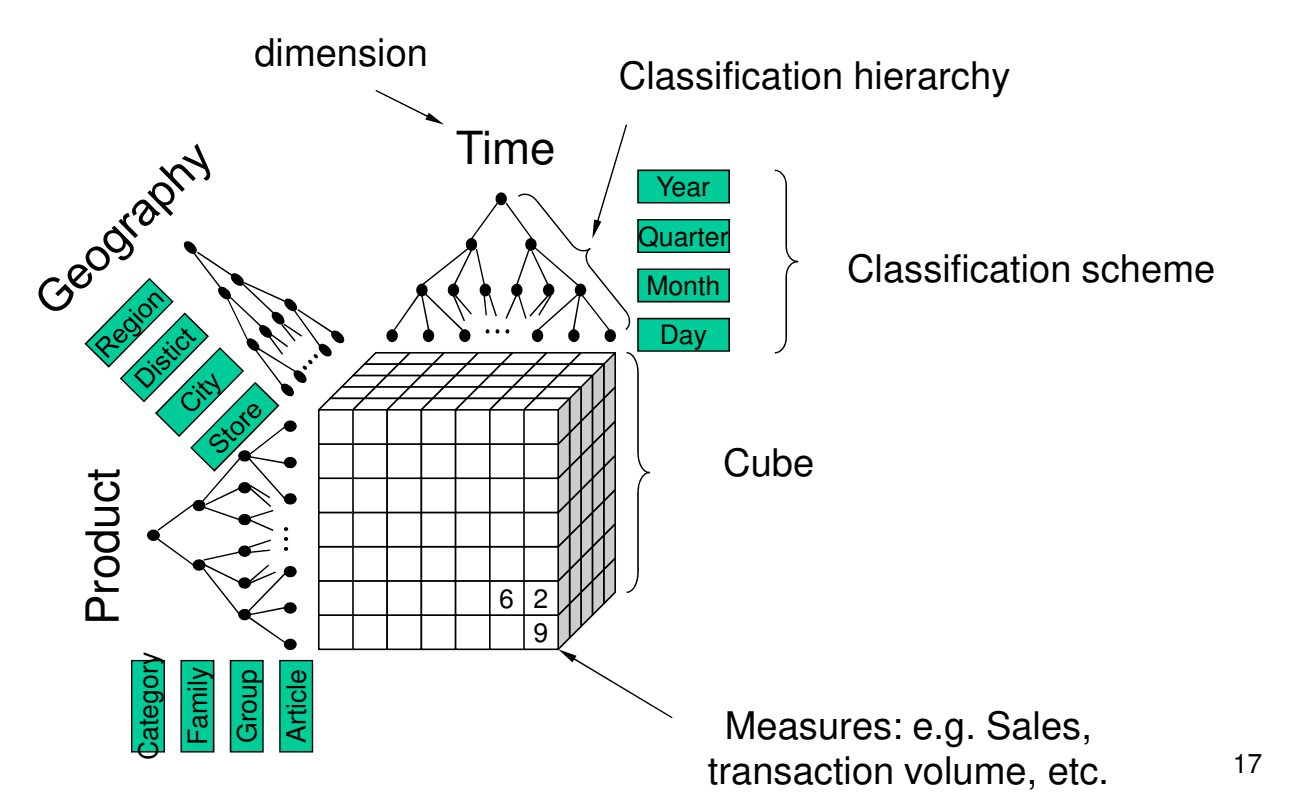
\includegraphics[width=0.8\textwidth]{cube.png}
    \caption{An instance of a data cube}
    \label{fig:cube}
\end{figure}

\subsubsection{Features of Measures}
Measures have a name, domain and aggregation type.
The domain is roughly equivalent to their data type, but restrictions are possible (e.g. negative cost).

Aggregation types are:
\begin{itemize}
    \item \textbf{FLOW:} arbitrarily aggregationable (Turnover, Sales)
    \item \textbf{STOCK:} not temporally summable (Stock)
    \item \textbf{Value per unit (VPU):} not summable (Price, taxes)
\end{itemize}

\subsubsection{Multi-dimensional Operations}
By representing our data as a cube aggregations become easy to understand operations:
\begin{itemize}
    \item \textbf{Pivoting:} rotate the cube along one or multiple axes
    \item \textbf{Roll up, Drill down, Drill across:} A roll up is the aggregation of data along one or multiple axes, a drill down is the opposite.
        A drill across performs analysis over a spectrum of dimensional values.
    \item \textbf{Slice and Dice:} this is just a visual representation of filtering
\end{itemize}

\subsubsection{Aggregation}
Aggregation is a change of granularity through some function.
Aggregation functions map a set of values to a single one, and can be done via cumulation (sums, averages) or ranking.

\textbf{Summability} of measures plays a huge role in aggregation, as it dictates which types of analysis are and aren't possible.
Disjunctivity, Completeness and Type Compatibility are necessary for aggregation.
Disjunctivity and Completeness are themselves necessary attributes of classification hierarchies.
Completeness means that all elements must be contained in the hierarchy, and Disjunctivity means no element can be contained in two classifications in the same hierarchy.
The type compatibility is dependent on the aggregation type of the variable in question.

\subsection{Schema Creation and Updates}
According to Kimball this should be done in four steps:
\begin{enumerate}
    \item Selection of business process
    \item Selection of the granularity
    \item Selection of the dimensions (useful for functional dependencies)
    \item Selection of the measures
\end{enumerate}
\begin{keypointbox}
    In my opinion one should select the dimensions before the granularity, but maybe that's just me
\end{keypointbox}

Schema updates are very tedious, as the metadata has to be kept consistent even with the schema changes.
The approach by Chamoni and Stock suggests versioning the classification hierarchies and storing the timestamps in a validity matrix.
The schema can also evolve, with most of it staying the same as the old version.
\textbf{This is dangerous territory.}

\section{Implementation of the MD Model}
We need to find a way of storing our MD model.
We could use a classical relational database, which would be very scalable, but we would have to transform all queries into relational form.

Alternatively we could create a multi-dimensional database, which would have easier querying, but would scale very badly due to empty cells.

We could also combine both approaches, giving us a tradeoff between the two.

\subsection{Relational Storage}
This requires three layers: an RDBMS (relational DBMS), storing the data and performing the queries, an OLAP server transforming the OLAP operations into SQL, and a presentation layer, which the user interacts with.

The problem is we have to find a suitable storage method while keeping the cardinality and consistent performance over all dimensions.
As a start, we define every cube cell via a single tuple.
This tuple contains the measure data and references to the dimension data.
There are multiple ways of storing the dimension data.

\subsubsection{Snowflake Schema}
The snowflake schema stores dimensional data in a tree of references.
An example is shown in \Cref{fig:snowflake}.
This schema is fully normalized, and has thus no memory overhead.
However, queries require joins over a lot of tables, making them slow (some DBMS optimizations can help here).

\begin{figure}[h]
    \centering
    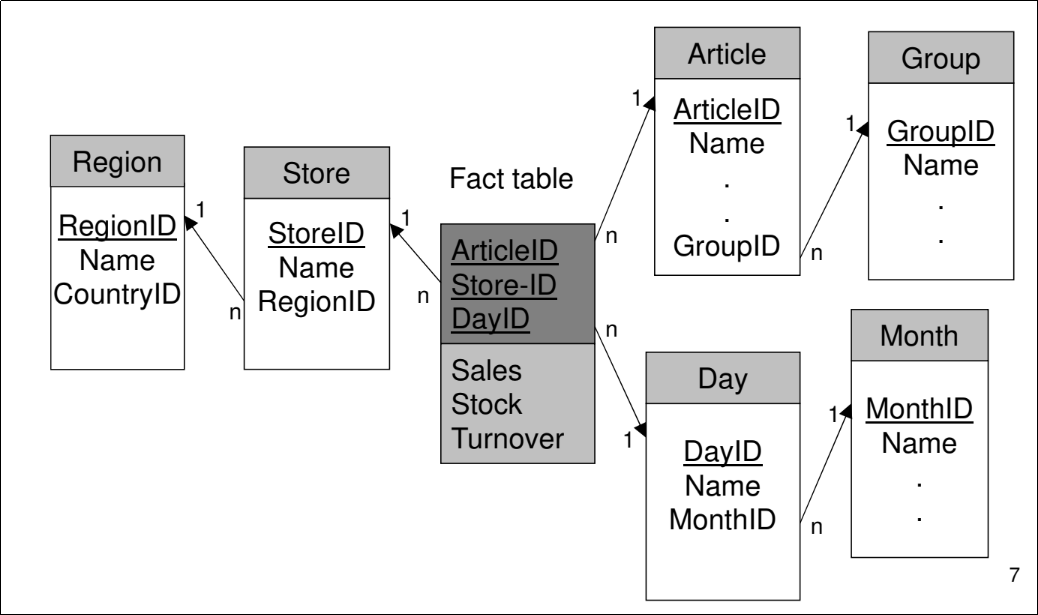
\includegraphics[width=0.8\textwidth]{snowflake.png}
    \caption{An example of a snowflake schema (the 7 is a page number)}
    \label{fig:snowflake}
\end{figure}

\subsubsection{Star Schema}
The star schema is basically a snowflake schema that is not normalized.
The data in the dimension tables is potentially very redundant, which can lead to increased memory consumption.
The joins in the query are faster (because there are fewer) with the star schema.
An example is shown in \Cref{fig:star}.

\begin{figure}[h]
    \centering
    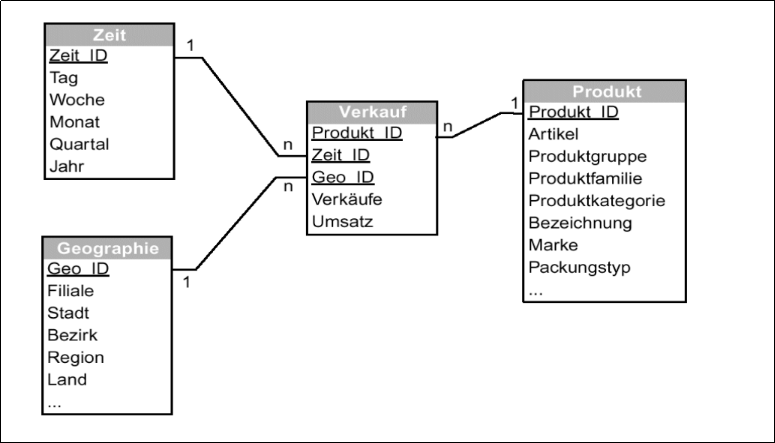
\includegraphics[width=0.8\textwidth]{star.png}
    \caption{An example of the star schema}
    \label{fig:star}
\end{figure}

\begin{keypointbox}
    If multiple cubes are necessary, just reuse and combine parts you already have.
    This leads to a galaxy representation
\end{keypointbox}

\subsection{MD Queries}
A common pattern is the star join pattern.
You simply join the fact table with the dimension table through the indices stored in the fact table.
Because grouping along multiple dimensions is a frequent use-case in DWs, modern DBMSs have special methods for that.
I will explain them in the order that I found easiest to understand.
All of this can be done with simple group by clauses and unions, but that is an absolute nightmare for larger numbers of tables, and should be avoided where possible.

\subsubsection{Grouping Sets}
A grouping set is used in the \lstinline{GROUP BY} clause of a query.
It is a set of sets defining the different groupings.
\Cref{fig:groupingset} shows a very good example of how they work (for anyone interested it was taken from the postgresql manual on grouping sets).

\begin{figure}[h]
    \centering
    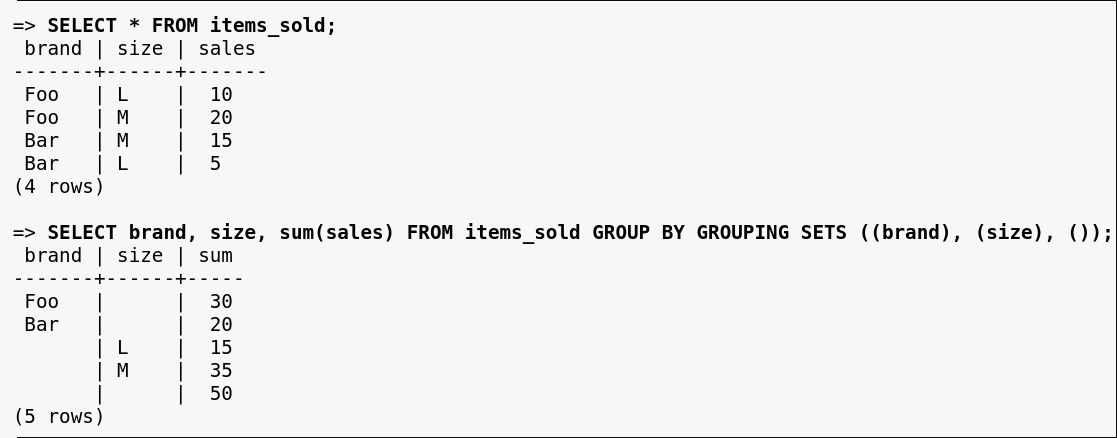
\includegraphics[width=\textwidth]{groupingset.png}
    \caption{An example of grouping sets}
    \label{fig:groupingset}
\end{figure}

\begin{keypointbox}
    A grouping set of $((a),(b,c),())$ will aggregate over rows with the same value in column $a$, then over all rows with identical $b$ and $c$ columns, and then over all.
    It will display all results in the same table.
\end{keypointbox}

\subsubsection{Rollup}
A rollup of $(a,b,c)$ is equivalent to a grouping set of $((a,b,c), (a,b), (a), ())$.
The rollup operator always adds the aggregate over all rows.
If this is not desired, the row should be filtered.

\subsubsection{Cube}
The cube operator calculates the power set of the supplied column set, and uses that as a grouping set.
For example, a cube of $(a,b,c)$ becomes a grouping set of $(a,b,c), (a,b), (a,c), (b,c), (a), (b), (c), ()$.

\begin{keypointbox}
    A \lstinline{ROLLUP} performs a rollup along a single dimension, a \lstinline{CUBE} does so along all combinations of dimensions.
\end{keypointbox}

\subsubsection{Other useful functions}
The \lstinline{GROUPING()} function tells us whether a given column was aggregated, and if multiple columns are supplied, it tells us the aggregations in a bitmask fashion.

There also usually exist nicer functions for handling date data-types.

\subsubsection{The \lstinline{OVER} Clause}
This clause allows us to include aggregations with the unaggregated data.
\Cref{fig:over} shows an example.
\lstinline{OVER} can also be used for window functions.
This is actually very well explained in the POSTGRES documentation, and a very nice example is shown in \Cref{fig:window}.
Window functions can also be used for ranking with the \lstinline{RANK()} and \lstinline{DENSE_RANK()} functions.

\begin{figure}[hp]
    \centering
    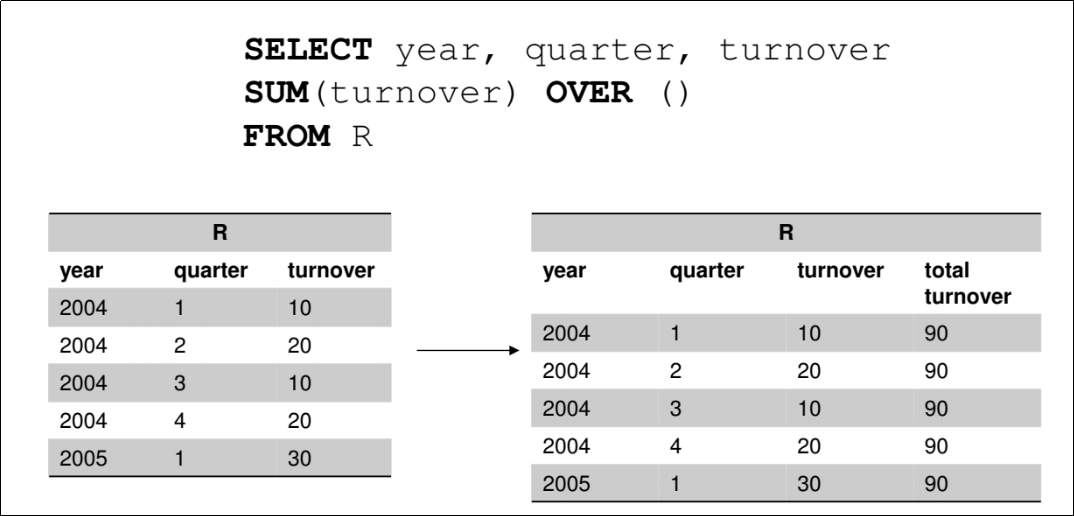
\includegraphics[width=\textwidth]{over.png}
    \caption{An example of the \lstinline{OVER} clause}
    \label{fig:over}
\end{figure}

\begin{figure}[hp]
    \centering
    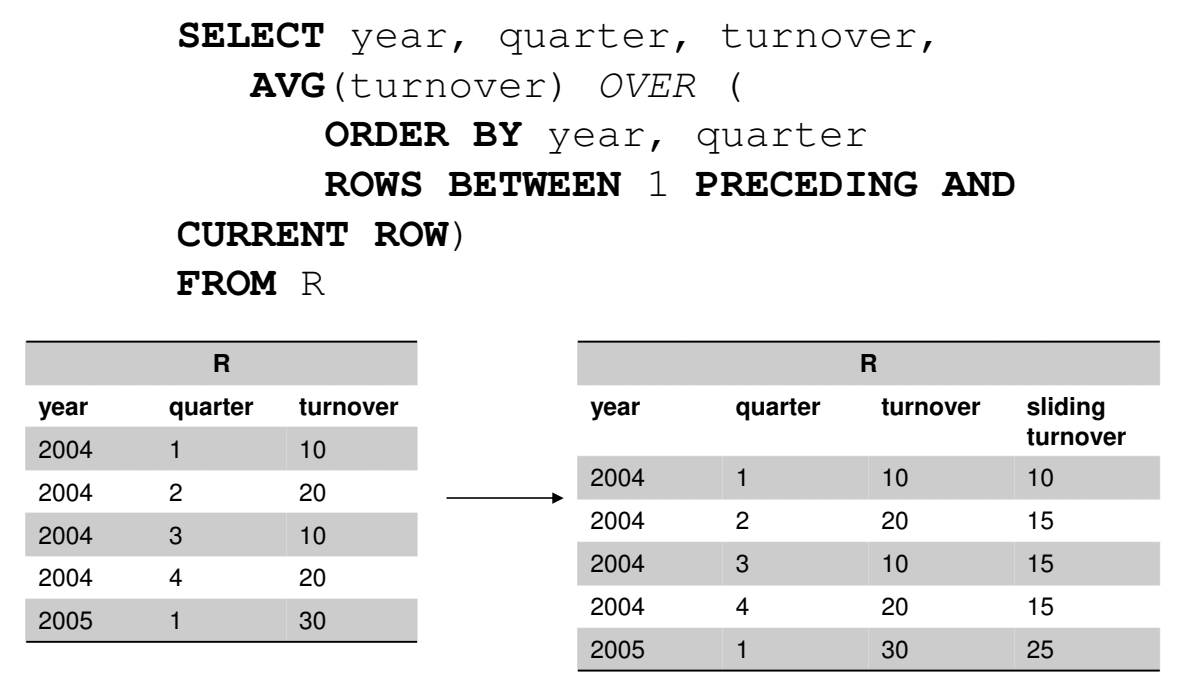
\includegraphics[width=\textwidth]{window.png}
    \caption{Using \lstinline{OVER} for sliding window computation}
    \label{fig:window}
\end{figure}

\section{Versioning}
Versioning can be very important in DWS systems.
For organizational or legal reasons, deleting entries can sometimes not be an option.
In those cases we need to add some measure of declaring a tuple invalid.

There are in general four methods of versioning:
\begin{itemize}
    \item Overwriting old values
    \item Adding a version number
    \item Tuple timestamps
    \item Attribute timestamps
\end{itemize}
Where overwriting old values leeds to data loss and is thus sometimes unacceptable.

Attribute timestamping adds a start and end validity date to every attribute (leading to non-first-normal-form tables), while timestamping saves a start and end date for every tuple.
Because we need the beginning and end time of both validity and the transaction, we need a total of four additional columns per timestamped attribute or tuple.
Adding timestamps to tuples can lead to significant memory overhead due to the redundant saving of unchanging tuple parts.

\subsection{Schema Updates}
Sometimes changes to the schema become necessary.
These are \textbf{a lot harder} to handle than instance updates, because they could force us to remodel the entire DW.
The two main methods of handling them are schema versioning and schema evolution.
For schema evolution old queries are still possible, but for a new schema this might not be the case.
The steps necessary for adapting a schema to certain changes are shown in \Cref{fig:changes}.

\begin{figure}[hp]
    \centering
    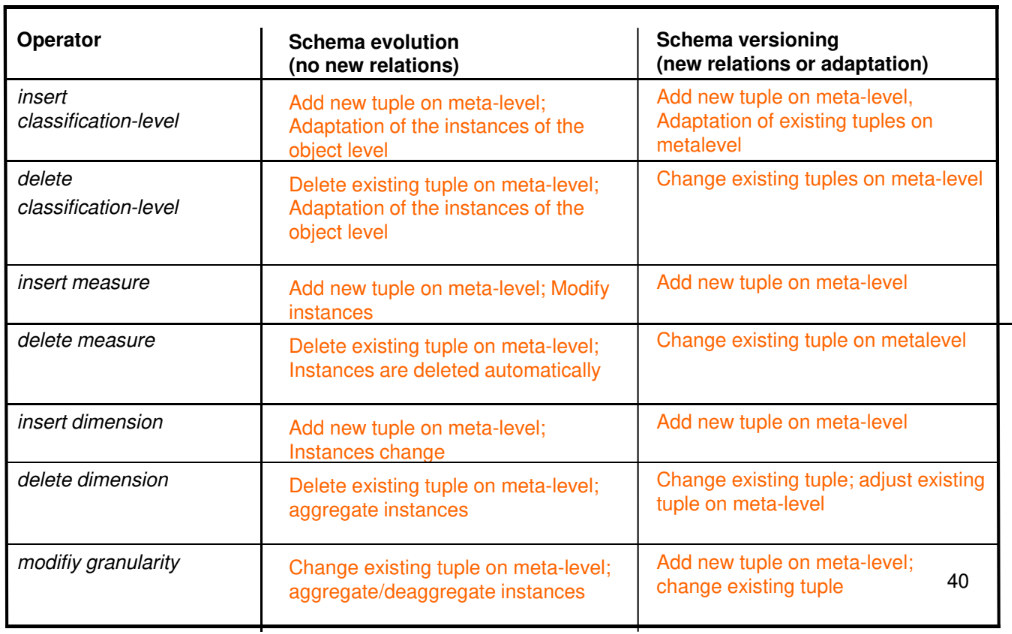
\includegraphics[width=\textwidth]{changes.png}
    \caption{Necessary steps for schema updates}
    \label{fig:changes}
\end{figure}

\section{Multi-dimensional Storage}
The best abstract model for storing things in MD fashion is a cube.
However, we do not only consider a three-dimensional cube, but an $n$ dimensional hypercube.
For visualization purposes we can reduce it to three dimensions, and our operations will work on other dimensions just the same.
We now need two (different) data structures for the dimensions (for addressing) and for the cube itself.

\subsection{Dimensions}
Abstractly viewed, a dimension is an ordered list of values (along that dimension).
These values have a fixed domain.
By ordering the dimension values we can create a mapping from dimension value to index and vice versa.
If we know all dimension values of a cell, we can then calculate its position in memory.
The order of the dimensions can be chosen arbitrarily and is fixed after setup of the data cube.
It has far reaching consequences concerning queries on the cube.

There are multiple ways for storing complex records in cubes:
\begin{itemize}
    \item \textbf{Complex cells:} These store the entire tuple of measures in the cell designated by the dimension values
    \item \textbf{Multiple cubes with flat cells:} Create one cube per measure ("Multi-Cube" approach)
    \item \textbf{Measure dimension:} Push (some) measures into the dimensions, requires all measures to be of the same data type
\end{itemize}

While single cube approaches are easier to understand, they can create large memory overhead because of large areas (volumes) in the cube with NULL values.
Multi-cube approaches limit this memory consumption, but require joins for data consolidation.

\subsection{Classification Hierachies and Aggregations}
An optimization approach is to store both the dimension values and all nodes of higher classification levels in the cube.
This means that all cells in a certain category are aggregated (for example during updates) and this aggregation is also stored in the cube, reducing the query time for future aggregations.
Such aggregations can also be done only for parts of the cube.

Unfortunately, this increases the size of the cube, which may or may not be an issue.
For small cubes it is better to just calculate these aggrgations at query time, while for larger cubes this can become vital.
Storing aggregations only for some hierarchy levels (e.g. every second) can create an optimal middle ground between both approaches.

\subsection{Partial and Virtual Cubes}
Query results for all queries on a cube are also cubes, thus allowing the same optimizations and techniques.
Also, views created on the cube are themselves (virtual) cubes and allow for the same processing as real cubes.

\subsection{Storing MD-data in MD-arrays}
A more direct approach to saving MD-data is saving them in arrays.
For any amount of dimensions we need to linearize the data for storage.
This makes storage very compact, compared to tables.
A large part of the performance stems from the order the dimensions are linearized in.
\Cref{fig:linearization} shows an example of such a linearization.

\begin{figure}[h]
    \centering
    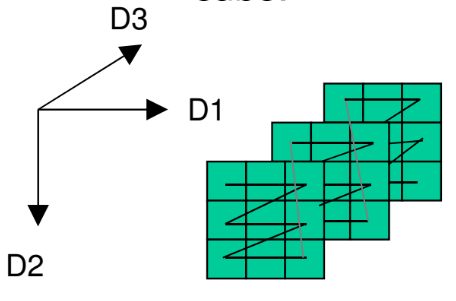
\includegraphics[width=0.4\textwidth]{linearization.png}
    \caption{An example of MD-array linearization}
    \label{fig:linearization}
\end{figure}

Calculating the index based on the dimension values is then very simple and follows the formula:
\begin{equation}
    I = \sum_{i=1}^n v_i \prod_{j=2}^i |D_{j-1}|
\end{equation}
So for three dimensions we get $I = v_1 + v_2 \cdot |D_1| + v_3 \cdot |D_1| \cdot |D_2|$.
Index calculation can be sped up using the Horner Schema.

\subsubsection{Sparse vs Dense Population}
The filling level is given by the number of filled cells, divided by the number of total cells.
Dense population is given when the filling level is high, sparse population is given when it is low.
For dense populations, array storage is more efficient than relational storage.
For sparse populations, we can make some adjustments to the array saving method to greatly increase storage efficiency.

One method is to not store empty areas in sparsely populated arrays.
If the empty cells would occupy an entire memory block, you can just skip it.
This requires additional calculations for indices.

There is also the possibility of storing sparsely populated dimensions on another level than densely populated ones.

\subsubsection{Limitations of MD-Storage}
\label{limitations}
MD-storage methods do have some limitations.
It can be expensive to maintain the full MD-array (due to null-values), and not saving NULL areas makes it more like a relational approach.
Inserting new values can cause \textbf{a lot} of memory shifting in order to keep the order on indices consistent.
There is also no current standard for MD-storage, as opposed to SQL, and all query languages are proprietary.

\subsection{Target Figures}
Target figures can be difficult to store in MD-arrays, as they are only known in spares quality (e.g. only per store per month), and need to be filled in later.
We would however still be able to calculate with them in aggregations (e.g. prognosing yearly totals for the running year).
This requires the DW to maintain the target figures itself, often with (goal) tracking.
The target figures can also be stored along with actual measures in the cube cells.

\subsection{Access Control}
Access control is a tricky issue for OLAP systems, as we want to generate accurate reports without the user obtaining specific information he or she should not usually access.
A user can also obtain specific cell values by using tracker queries and set algebra.
An example of a tracker query is shown in \Cref{fig:tracker}.
Most systems only have a simple rights system which does not protect against tracker queries.
A possible countermeasure would be to recognize tracker queries and forbid the user from accessing the results.
This could however disrupt the workflow and make generating all desired reports impossible, due to queries resembling tracker queries by chance.

\begin{figure}[h]
    \centering
    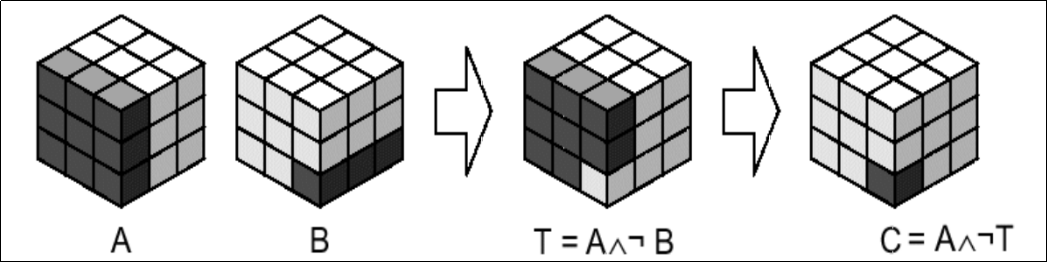
\includegraphics[width=\textwidth]{tracker.png}
    \caption{An example of tracker queries}
    \label{fig:tracker}
\end{figure}

\section{Index Structures for the MD data model}
As covered briefly in \Cref{limitations}, we want our data structure to support certain operations efficiently.
Because we cannot move the \textbf{entire} DW on inserts (and for other performance reasons), we cannot use native MD-arrays as storage method.
As relational storage methods have become the norm, and with that highly optimized, they are also used for DWs.
In order to use them efficiently for DW queries (range queries, aggregations, ...), we need to do some optimization on the index structure.

We want to store our data in a way, such that data which is in close proximity to each other in \textbf{any} dimension is in close proximity in memory.
This greatly reduces the number of disk accesses we need for range queries, as it increases the likelihood of tuples being on the same memory block.
As memory controllers access one memory page at a time anyway, having more tuples on the same page decreases query time.

Index structures can be classified as follows:
\begin{itemize}
    \item \textbf{Clustering:} Clustering index structures keep neighboring tuples in close proximity in memory.
        We can further distinguish between tuple clustering (tuples are clustered on a memory page) and page clustering (pages are stored in tuple order).
        Page clustering is very expensive, as it requires page reordering; however, it allows for prefetching in queries.
        In non-clustering index structures the tuples are stored in random order.
    \item \textbf{Dimensionality:} States the number of attributes of the underlying relation used for calculating the index key.
    \item \textbf{Symmetry:} In symmetrical index structures the order of index attributes is not relevant for performance of the index structure.
    \item \textbf{Dynamic Behaviour:} The cost of updating the index structur on dynamic changes.
\end{itemize}

The following subsections will cover the index structures.
I will not go into too much detail, but will rather provide a refresher.
Most of the index structures are actually very intuitive, and most of them are very well explained by wikipedia.

\subsection{B-trees}
B-trees are used in regular OLTP databases.
They provide a method for generating a \textbf{guaranteed balanced tree} with low depth.
Insertion in B-trees is fairly simple.
You add the new element where it would belong (by order of its primary key), and if the node is full, you split it, moving the middle element to the parent node.
If there is no parent node, you create one.
An example is shown in \Cref{fig:b_tree}.

Deleting from a B-tree is done by removing the elemnt from its containing node.
If the node is now too empty, we combine it with one of the neighboring siblings.
This might cause a split and a reorganization of the index structure, which makes deleting from B-trees tedious.
Luckily, this is a non-issue in DWs, as we never really delete anything.

\begin{figure}[h!]
    \centering
    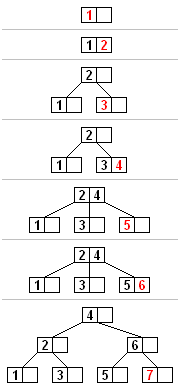
\includegraphics[width=0.6\textwidth]{B_tree_insertion_example.png}
    \caption{An example of insertion into a B-tree}
    \label{fig:b_tree}
\end{figure}

\subsubsection{B*-trees}
In order to achieve greater in order traversal speed, we push the elements all into the leaves, with the internal nodes only acting as organizers.
If we now store a reference to the next (and previous) leaf node in every leaf, we can get very high in order traversal speed.

\subsubsection{Problems with B-trees}
B-trees can only work with a single index.
Even when combining multiple dimension values into a single index like in MD-arrays, we can only efficiently traverse them in a single dimension.
B-trees are \textbf{asymmetrical}.

\subsection{Grid-Files}
Grid files are essentially a grid of references to buckets.
The dimensions of the (n-dimensional) grid represent the domain of the dimension values in our DW.
After calculating the position of the element in the grid via the dimension values, the element is stored in the bucket referenced at the target location.
Because the buckets are limited in size, splitting might become necessary.
This is done by splitting the grid row (or column or n-dimensional equivalent) into two halves, and creating a new bucket.
All non-full buckets in the same row can stay as they were, as we can simply replicate the reference to them.
This means that once we split a bucket in a row, all other buckets in the same row now have two references to them.
Should one of them also become too full, we can create a second bucket without splitting the row again.
If a bucket becomes empty we can simply combine it with the "neighboring" bucket, and store the same reference in two grid cells.

Row splitting in grid files is an expensive operation, as all other references have to be moved in memory for the grid file to stay performant.
Apart from this performance issue, they offer great clustering and symmetry properties.

\subsection{R-trees}
R-trees are optimized for elements that cannot be accurately represented as a single point.
It is mainly used for geographical objects (in 2-D, 3-D or n-D), but can be used for arbitrary multidimension data.
They work as follows:
Each leaf node approximates its represented element via its bounding rectangle.
Each intermediate node represents its children via their bounding rectangle.
These bounding rectangles are generally not disjunct, and so traversing multiple paths through the tree might become necessary for queries.
Each node contains between $m$ (lower bound) and $M$ (upper bound) elements.
\Cref{fig:r-tree} shows an example of an R-tree and its 2-D representation.
Because the branching in every level is at least $m$, the height of the tree is bound by the logarithm to base $m$.

\begin{figure}[h]
    \centering
    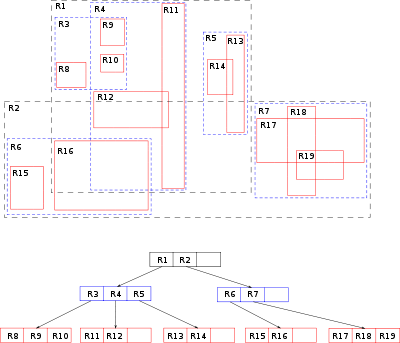
\includegraphics[width=\textwidth]{r-tree.png}
    \caption{An example R-tree with $m=2$ and $M=3$}
    \label{fig:r-tree}
\end{figure}

\subsubsection{Algorithms for R-trees}
\paragraph{Searching} is done by traversing the tree and selecting path(s) whose bounding rectangles contain the search point.
For range queries the same thing is done but with intersections with the search rectangle.

\paragraph{Insertion} works almost the same way as in a B-tree.
However, due to the potentially overlapping bounding rectangles, multiple candidates must be considered.
The candidate which requires less increase in their bounding rectangle is chosen.
Just like in B-trees, if a node is overfull, this causes a split.
Splits are a bit more complex than in B-trees, and will be covered separately.

\paragraph{Deletion} is done by simply removing the element from its containing node, and adjusting the bounding rectangle.
If changes occur, they are propagated recursively upwards.
Should an underflow happen we can combine sibling nodes.
As opposed to B-trees, any siblings can be combined in R-trees.
The combination with the smallest increase in bounding rectangle is chosen.

\paragraph{Splitting} is a non-trivial problem, as finding the best way to split is expensive.
There exists a quadratic algorithm which solves this.
In the first step, all pairs of children are tested for their wastefulness, and the most wasteful pair is chosen as seeds for the new split nodes.
(Wastefulness is calculated by the difference of the bounding rectangle area and the individual rectangle areas).
This guarantees us a maximum distance between the seeds.
Now we simply take a random other child and add it to the node where it causes the lesser bounding rectangle increase.

There is also a heuristic linear cost algorithm, which works almost the same way but chooses the seeds differently.
For each dimension, it records the normalized separation between the lowest high side and the highest low side.
It then chooses the rectangles which have the highest separation along any dimension.
The comparison is possible because the distances have been normalized (divided by the total length of the set along their respective dimension).

A very good graphic example can be found on the slidedeck for chapter 5, on pages 49 to 70.

\paragraph{Evaluation of the R-tree}
R-trees are a dynamic, height-balanced structure which is suitable for storing large amounts of data.
If the data is distributed "well", they can provide rapid access.
Well in this case means distinct boinding rectangles.

The rectangle approximation however can be rather imprecise, and the quality and speed of the search space is limited by the overlap of the rectangles.
In the worst case the entire index space has to be searched.
Update algorithms are also very costly, which makes R-trees not ideal for data which is highly dynamic.

\subsection{R\textsuperscript{+}-trees}
These trees solve the search space overlap problem by "clipping" the bounding rectangles.
If an element is contained in both rectangles, it (or a reference to it) is stored redundantly.
A graphical example is shown in \Cref{fig:r+-tree}. 
The elements are logically "cut" on insertion.
Due to the redundant storing of elements, additional memory overhead can be incurred.
This is somewhat balanced by the reduced query time, but the query time can also be reduced in different ways.

\begin{figure}[h]
    \centering
    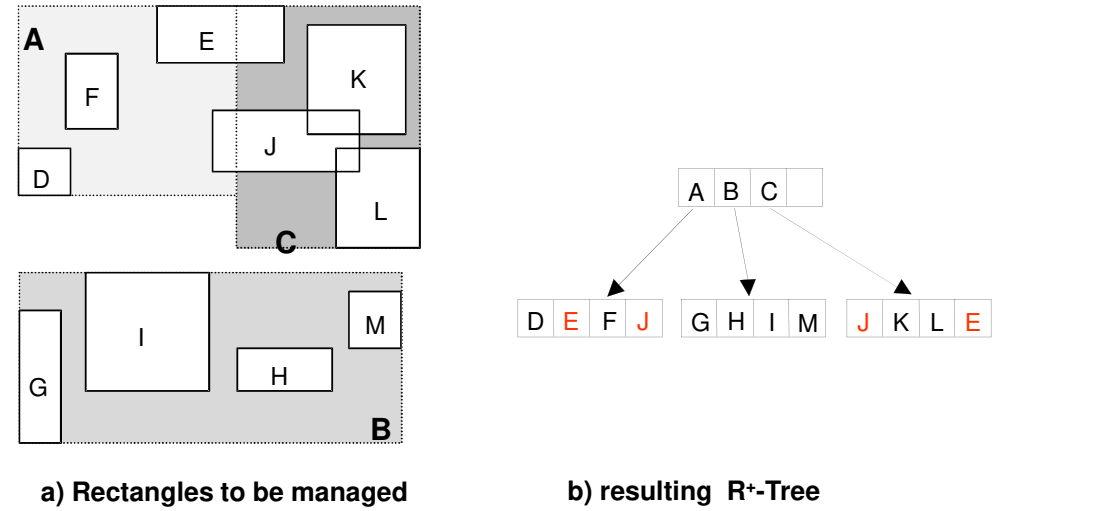
\includegraphics[width=\textwidth]{r+tree.png}
    \caption{A graphical example for an R\textsuperscript{+}-tree}
    \label{fig:r+-tree}
\end{figure}

\subsection{R*-trees}
By doing some optimizations with the insert and split algorithms we can get performance comparable to the R\textsuperscript{+}-tree without the redundant saving.
We want to minimize the area of the bounding rectangles and the overlap and circumference of search space rectangles.

\subsubsection{Insertion}
While inserting we calculate the candidate nodes for the new element based on the area increase.
This is done for every pathing decision during the downwards traversal of the tree.
This increases the complexity of the insertion somewhat, but gives us much better query performance.

\subsubsection{Splitting}
First the best axis for splitting along is chosen.
This is done by sorting all elements by their highest and lowest border in all directions.
These sorted lists are then split in the middle, and the sum of circumferences of the resulting bounding rectangles is calculated.
The axis with the lowest circumference is chosen.

Along the chosen axis, all distributions are tested, and the distribution which results in minimal overlap is chosen.

\subsubsection{Forced Reinsert}
In order to still achieve good search space organization independent of insertion order, there exists the possibility of performing a reinsert on node split.
All this does is choose a number of (random) elements after the node split and reinsert them.
Because these nodes might be inserted in different parts of the tree, potential new splits might arise.

\subsection{UB-trees}
UB-trees were designed to cluster tuples on disk space while preserving close proximity.
They provide efficient incremental organization (they work fast after updates) and give logarithmic worst-case guarantees for insertion, deletion and point queries.
Range queries are also handled efficiently, and memory utilization is good on average.

\subsubsection{Z-Ordering}
Z-ordering is a way of ordering tuples in memory.
The Z-index is calculated as follows:
\begin{equation}
    Z(x) = \sum_{i=0}^{s-1} \sum_{j=1}^d x_{j,i} \cdot 2^{i \cdot d + j -1}
\end{equation}
The meaning of the variables is not really explained anywhere in the slides, and I personally believe that Z-ordering is much better understandable if it is shown as in \Cref{fig:z-order}.
They are basically just fractal Zs, if that makes sense.

\begin{figure}[p]
    \centering
    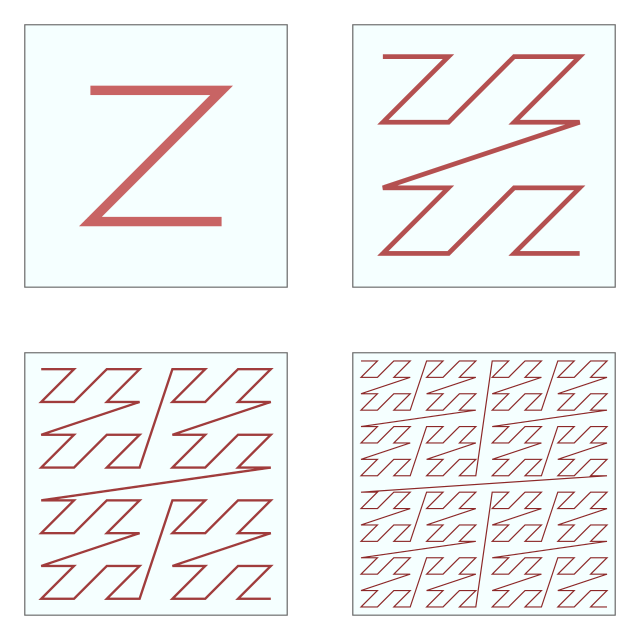
\includegraphics[width=0.8\textwidth]{z-order.png}
    \caption{Four Z-curves with different granularity}
    \label{fig:z-order}
\end{figure}

\paragraph{Z-regions} are regions in Z ordering given by a start and end index.
They can be interpreted both as "linear" intervals on the Z-curve or as geometrical regions in the multidimensional plane.
\Cref{fig:z-region} shows the different interpretations.
Because there exist efficient conversions between Z-order and tuple values and vice versa (bit interleaving) we can arbitrarily switch between both interpretations of Z-regions.

We can represent memory pages with Z-regions, and can thus quickly calculate which memory pages are relevant for a range or point query.
The rightmost image in \Cref{fig:z-region} shows a possible point entry distribution for the Z-regions of the middle image with a memory page capacity of two entries per page.
The Z-regions of a UB tree are stored in a B-tree, and can thus efficiently be found.

\begin{figure}[p]
    \centering
    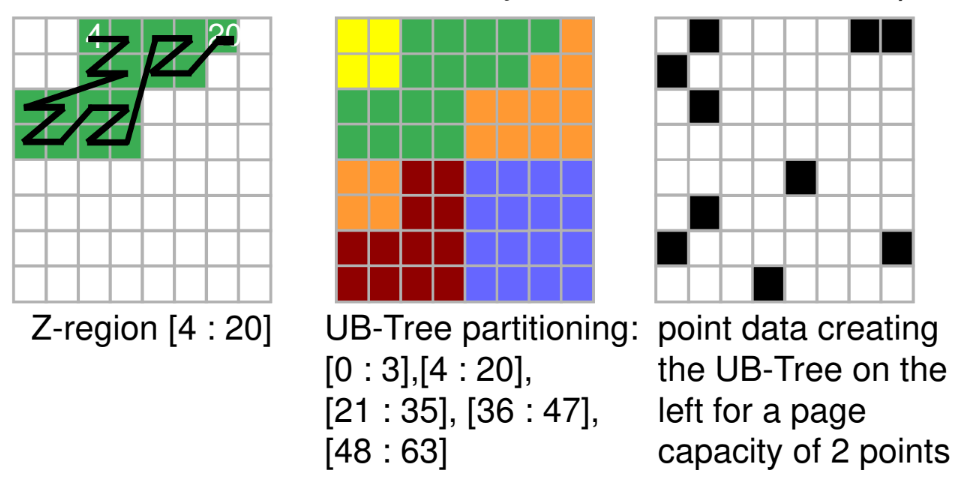
\includegraphics[width=0.9\textwidth]{z-region.png}
    \caption{Different interpretations of Z-regions}
    \label{fig:z-region}
\end{figure}

\subsubsection{Insertion}
By calculating the Z-index of a tuple upon inserting we can quickly find the memory page (Z-region) it belongs to.
If there is no space left on the memory page for the new entry the Z-region has to be split.

\subsubsection{Range queries}
We calculate the bounding box of the search box in Z-space.
Then we find all intersecting Z-regions, load the tuples from them and select the ones within the search box.

\subsubsection{Tetris algorithm}
In order to improve memory requirements for range queries (and a few other performance improvements) the Tetris order and algorithm were introduced.

The elements and Z-regions are traversed in vertical or horizontal slices in geometrical space.
This reduces the worst case memory requirements for the search to linear in the size of the result set, not the entire database.

Z-regions are added until a full slice is cached, then the required elements are added to the result set.
All Z-regions that do not pass over into a slice that has not been processed are then removed from the cache, and the next slice is processed.

\subsection{Bitmap Indices}
As tree structures degenerate with an increasing number of dimension, people have looked for alternative datastructures.
One idea has been to use dimensions of low cardinality (ideally booleans) as a bitmap.
This gives us a bitmap vector for every column, and filtering upon these vectors is easy.

Encoding dimensions of higher cardinality is quite difficult however.
For example, to encode the month of birth we need twelve bits for a bitmap instead of four for a regular integer.
For the day of birth (from 0 to 365) we would need $365/8 = 46$ byte of memory \textbf{per tuple}.
This can become too much very quickly.

Also, because bitmaps are non-clustering index structures the time to access all filtered tuples can be quite large.
This makes bitmaps better for small result sets.
Updating them is also inefficient, but this is acceptable for DWs, as updates are not frequent.

\subsubsection{Multicomponent Bitmap Indices}
To reduce the problems arising from this, one can encode values of higher cardinality using their binary representation.
This reduces the memory requirement from linear to logarithmic in the cardinality.
Using this method has the drawback that most indices still have to be accessed in order to get the result set.
Any other encoding than binary can also be used, but binary is used in the internal representation anyway.

\subsubsection{Range-coded Bitmap Indices}
Setting the bitmap value to 1 not only if the value matches, but if the value is less than or equal (or the other way round) than a certain (fixed) threshold makes bitmap indices better for range queries.
The tradeoff here is that we either lose match query performance or incur additional memory overhead.

Range-coded bitmap indices can be combined with multicomponent indices.

\subsubsection{Interval-coded Bitmap Indices}
By encoding whether or not a value is in a certain interval range queries can be accelerated as well.

\subsection{Partitioning}
Partitioning can work like an index structure, and it can be combined with index structures.
It is the process of splitting a relation into autonomous sub-relations.
All sub-relations combined form the master relation.
Relations can be partitioned either horizontally or vertically.
Both strategies are shown in \Cref{fig:partitioning}.

\begin{figure}[hp]
    \centering
    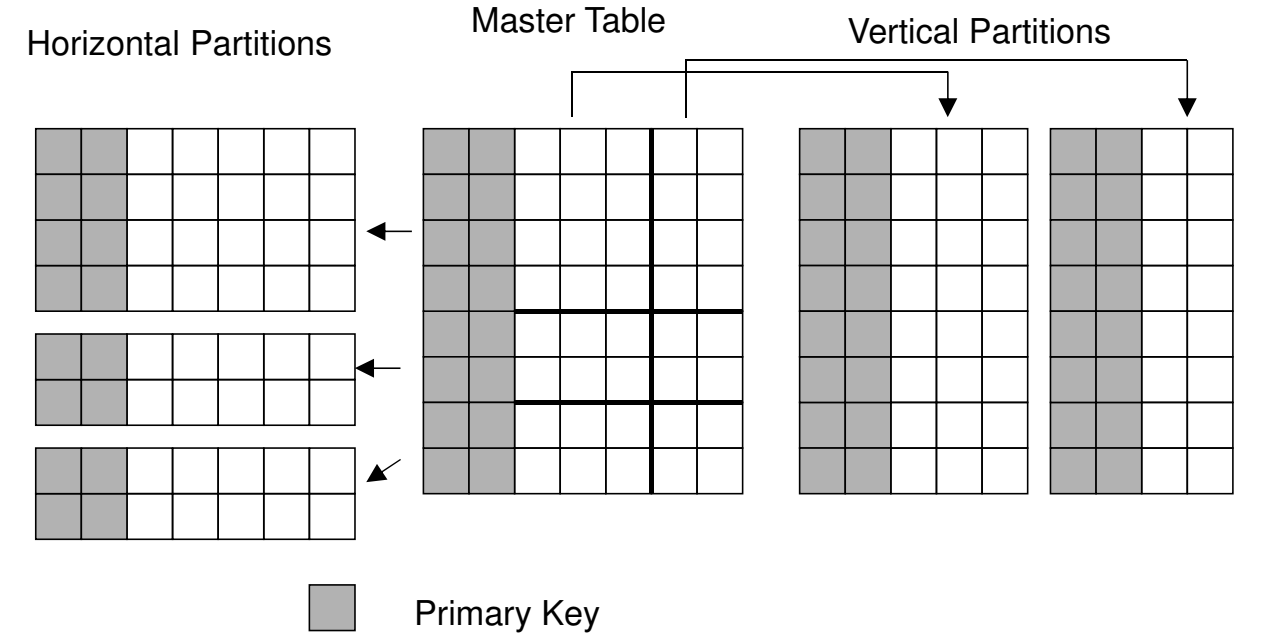
\includegraphics[width=0.8\textwidth]{partition.png}
    \caption{Partitioning strategies}
    \label{fig:partitioning}
\end{figure}

\subsubsection{Horizontal Partitioning}
A relation is split into a set of pairwise disjunct set of sub-tables.
Attributes for all sub-tables are the same.
The two ways of doing horizontal partitioning are range based and hash based.

\paragraph{Range based partitioning} is commonly done as it is very easy.
The rows are split into sub-tables based on their values for certain attributes (e.g. all washing mashines).
Tailoring the splitting criteria to the frequency of queries gives the highest performance boost.
If, for example, half of my queries are concerned with the sales in Austria only, it makes sense to move all values for Austria to their own sub-table.
Because values are \textbf{actually physically moved} during partitioning, this greatly increases the query time due to now given proximity in memory.
A typical partitioning criterium is time, as normally newer values are more interesting.

\paragraph{Hash based partitioning} partitioning based on the hash of a value or a combination of values balances the load, due to the nature of (good) hash functions.
This technique is seldom used as random tuples will be grouped together, which usually results in bad query performance.
It can be useful if most queries are aggrigates over all data, but even then partitioning based on some other attribute is better because it is more intuitive.

\subsubsection{Vertical Partitioning}
Storing certaing columns separately can have benefits for queries.
This is especially true if some attributes are queried very seldom, or very often, or there attributes that are usually not queried together.

The sub-tables store the primary key, and have a 1:1 relation to each other.
Combining them requires a join.

Splitting off attributes that are very rarely required can lead to the creation of mini-dimensions, leading to a reduced dimension table size.

\section{Star Join Optimizations}
As the star join required for classical star or snowflake schema DWs is very inefficient when using regular join techniques, some optimizations have been made.

One solution is calculating the cross product over the dimension tables, as these are relatively small.
This then requires only one big join with the fact table.
Using the cross product technique can get out of hand quickly for slightly larger dimension tables (e.g. three dimensions with 1.000 rows each gives 1.000.000.000 tuples).

Another technique is to first find the foreign keys that are required for the current query.
This is done with the dimension tables directly.
The fact table is only joined with the filtered result, leading to much smaller joins.

\section{Materialized Views}
Because most queries reference the same aggregations (e.g. sums of sales per month per store) it can become quicker to just store these results in memory.
While this greatly decreases query time, it does require extra memory.
Also, because the aggregated data is saved as a redundant copy, there might be some consistency issues on data changes.
For DWs this should be a non-issue, as we usually don't have updates, but this should still be kept in mind.

Another potential issue arises from the selection of materialized views.
Selecting the optimal aggregations to store is a hard problem.
Also not all parts of queries can be stored in materialized views.

\subsection{Usage of Materialized Views}
Materialized views are constructed by replacing parts of common queries with precalculated results.
Should be done only in cases where fetching from the materialized view is substantially faster than calculating on the fly, and worth the memory usage.
Also, if the existing views do not exactly match a branch of the operator tree, the query execution plan (QEP) has to be adjusted.
This raises more questions about the cheapest solution.
A general rule is avoiding accesses to the fact tables.

\subsubsection{Monoblock Queries}
Monoblock queries are regular star join queries (joining the fact table with the dimension tables).
These can easily be replaced by materialized views.
In general we replace the grouped selection from the fact table (joined with dimension tables) by a distinct selection from our materialized view.

In general, a Query $Q$ can be represented by another query $Q'$ on a materialized view $M$ iff (if and only if):
\begin{itemize}
    \item Selection conditions on $M$ are not more restrictive than those on $Q$
    \item Grouping Attributes for $Q$ have to be a subset of $M$
    \item If $Q$ contains aggregation functions, they have to be combinable from the aggregation functions in $M$
        \begin{itemize}
            \item if $Q$ contains sum then $M$ must contain sum
            \item if $Q$ contains average then $M$ contains either average or sum and count
        \end{itemize}
    \item Additional selection conditions in $Q$ must be applicable to $M$
\end{itemize}

\subsubsection{Multiblock Queries}
We want to extend the previous technique to arbitrary queries and views, even if the restriction on $M$ is stricter than that on $Q$.
This can be done by retrieving facts missing in $M$ from the fact table.
In general, the way to do this is by splitting $Q$ into selection criteria contained in $M$ and not contained in $M$.
We then perform a union of $M$ with the additional facts.
Because retrieving the missing facts can be quite complex, based on the restrictions on $M$, including the materialized view at all can have a negative performance impact.

\subsection{Additivity of Aggregation Functions}
Informally, a function is semi-additive if it can be calculated from the results of some other aggregation function (e.g. the average can be calculated knowing the sum and count of subsets).
If it can be calculated from results of itself, then it is additive.
A few examples:
\begin{itemize}
    \item \textit{sum} is an additive function
    \item \textit{average} is a semi-additive function
    \item \textit{count} is a semi-additive function (the global count is the sum of the individual counts)
    \item \textit{min} and \textit{max} are additive functions
\end{itemize}

\subsection{Selection of Materialized Views}
Selecting the optimal set of materialized views is hard (NP-complete).
The lecture slides describe multiple heuristics, as well as proposing static selection using intuition.
This part does not seem to be too important for the lecture, as it is not contained in the summary at all.

\subsection{Update of Materialized Views}
Materialized views can either be regenerated (which is potentially costly), or updated incrementally (which requires the calculation of deltas).
If the selction criteria of the update query are applicable to $M$ then the update on the fact table can simply be run on the materialized view as well.

If Up-to-dateness is not a pressing issue the views can also just be regenerated over the weekend or during other downtime.

\section{Data Mining}
The basic idea of data mining is to discover "knowledge" from existing.
This is mostly done by finding patterns in the sales data.

Data mining is an iterative process consisting of the following steps:
\begin{enumerate}
    \item Selection of data from the data basis
    \item Preprocessing: removing errors or incomplete values (this should be already done in a DW)
    \item Transformation: decreasing quantity
    \item Removing attributes rarely or never occuring
    \item Transformation into an analytical data basis
    \item Data Mining: the method used is defined by the goal
    \item Interpretation and Verification
\end{enumerate}

\subsection{Data Mining Methods}
\begin{itemize}
    \item \textbf{Dependency Detection:} finding statistical dependencies in the data set via either association rules or probability networks
    \item \textbf{Classification:} finding data points indicating a certain outcome (e.g. risk assessment for insurance companies)
    \item \textbf{Clustering:} splitting the data set into clusters of related data points
    \item \textbf{Sequence Analysis:} searching for frequently occuring episodes of events in time-ordered datasets
    \item \textbf{Regression:} detection of cause-effect relations between data points
    \item \textbf{Generalization:} generalizing new data points from an existing data set (e.g. interactive extrapolation)
\end{itemize}

\subsubsection{Clustering}
Here only the k-means algorithm is covered.
For k-means, $k$ data points are chosen as prototypes at random from the dataset.
Then we iteratively add new data points to the cluster closest to them.
We then move the prototypes to the mean of their respective cluster and repeat this until no data point is unclustered, all while minimizing the global distance of data points from their respective prototype.

\subsubsection{Classification}
In the lecture, only decision trees in the form of \textit{ID3} are covered.
Decision trees work by calculating the observed probabilities and conditional probabilities of the classification variable $c$ based on other attributes.
For decision trees, attributes of low cardinality are best, as the classification gets harder otherwise.
The shown method works as follows, and is a general approach to decision trees:
\begin{itemize}
    \item Pick the attribute $a$ which gives us the highest \textit{information growth} (limits the vulue of $c$ the most)
    \item Split the data set into (disjunct) sets of different values for $a$
    \item Repeat
    \item If no more attributes are left, add leaf nodes with the probability of $c$ for the current branch
\end{itemize}
If there is no $a$ that limits the value of $c$ significantly enough, there is the possibility of stopping short.
Decision trees have a problem of overfitting, as they fit the classifier very strongly to the training set.

\subsubsection{Association Rules}
Oftentimes in data mining we want to find dependencies in our data set.
This is used in many applications, e.g. recommending videos on YouTube or songs on Spotify.
While it is impractical to test all combinations of transactions, we can test those that show a minimum support
Association rules take the shape of $X \rightarrow Y$ and $X$ is the rule head, and $Y$ is the rule body.

\paragraph{Support} is the ratio of transactions containing a certain item.
Support for association rules is the number of transactions where the items of the rule occur together.
This can also be seen as the probability of the association rule "showing" (occuring).
\begin{equation}
    Sup(X\rightarrow Y) = {P(X, Y)} = \frac{\#(T\textup{ with } X,Y)}{\#(\textup{All transactions})}
\end{equation}

\paragraph{Confidence} is the ratio of the support of the assoction rule over the support of the rule head.
It can also be seen as the conditional probability of the rule given the rule head occurs.
\begin{equation}
    Conf(X\rightarrow Y) = \frac{P(X, Y)}{P(X)}
\end{equation}

\paragraph{Apriori Algorithm} works as follows:
\begin{itemize}
    \item Find all elements with support above a given threshold and add them to a set of association rules
    \item Append every element to every rule head in the set
    \item Remove the rules that are below a confidence or support threshold
    \item Keep the rules, and add them to the set of rule heads
    \item Repeat until the set of rule heads is empty
\end{itemize}
There exist more performant methods for finding association rules.
Filtering based on support from the beginning can remove a lot of rules from our knowledge base, but it saves us from computing trivial rules and rules that are worthless because they rarely occur.

\subsubsection{Summary}
Data Mining is a powerful method of gathering business intelligence.
The biggest problem of data mining is scalability, which is why many firms have specialized in running compute farms for data mining.
Also a lot of data mining services exist.

\end{document}
